\chapter{Primjena protokola za sigurno dogovaranje u okolini Interneta stvari}
\label{ch:iot}

Okolina Interneta stvari predstavlja mnoštvo uređaja različitih mogućnosti koji
su povezani putem Interneta i služe za pružanje raznih usluga, a temelji se na
vjerodostojnom prikupljanju podataka i pouzdanom upravljanju uređajima unutar
okoline.

Uređaji koji komuniciraju u okolini Interneta stvari često raspolažu ograničenim
mogućnostima. Temeljne mogućnosti uređaja Interneta stvari su:
\begin{itemize}
    \item vrsta i trenutna razina izvora napajanja,
    \item propusnost i kvaliteta mrežne povezanosti i
    \item računalna snaga na raspolaganju.
\end{itemize}

Uređaji u okolini Interneta stvari moraju biti u mogućnosti međusobno sigurno
komunicirati i pružati određenu razinu usluge. To se postiže s pomoću
sigurne komunikacije. Sigurna komunikacija zasniva se na prilagodljivom
dogovoru kriptografskih algoritama i potrebnih ključeva, koji je izveden u
sklopu
predloženog protokola ACAP. Uz protokol se koriste dodatne operacije zaštite
koje koriste rezultate protokola ACAP (dogovorene kriptografske ključeve i
algoritme) kao ulaz za zaštitu podataka ovisno o potrebnoj razini zaštite.

\section{Primjene sigurne komunikacije u okolini Interneta stvari}
\label{sec:scenarios}

Okolina Interneta stvari može se definirati kao slojevita arhitektura koja povezuje
razne uređaje kroz različite mrežne okoline. Cjelokupna arhitektura prikazana je
kroz par ključnih scenarija na slici \ref{fig:iot}, a temelji se na arhitekturi
predstavljenoj u \cite{perera2014context}. Cjelokupna arhitektura sastoji se od
tri osnovna sloja:

\begin{itemize}
\item \textit{Senzorski sloj} predstavlja izvor podataka cijele arhitekture, a
    čine ga uređaji ograničenih računalnih sposobnosti koji prikupljaju podatke
    iz okoline ili obavljaju jednostavne poslove.
\item \textit{Srednji sloj} se koristi za prikupljanje podataka iz senzorskog
    sloja i njihovo prosljeđivanje u gornji sloj računalnog oblaka. Uređaji na
    ovom sloju raspolažu s više resursa i mogu obavljati filtriranje i
    grupiranje podataka srednjeg sloja prije prosljeđivanja.
\item \textit{Sloj računalnog oblaka} predstavlja sloj usluge na kojem se
    obrađuju i skladište podaci koji se prikupljaju u senzorskom sloju, a
    filtriraju u srednjem sloju. Podaci obrađeni na ovom sloju koriste se za
    pronalaženje novih informacija na temelju kojih se upravlja ostatkom
    arhitekture u cilju ostvarivanja kompleksnih usluga upravljanja
    arhitekturom.
\end{itemize}

Osnovne primjene sigurne komunikacije prikazane su na slici \ref{fig:iot}, a
dijele se u četiri osnovne kategorije. Zaštita komunikacije ključna je za
sigurnost cijele platforme kako bi se omogućila provjera autentičnosti
izvora podataka i zaštitila komunikacija između uređaja koja predstavlja temelj
cjelokupne okoline Interneta stvari.

\begin{figure}
    \captionsetup[subfigure]{aboveskip=4pt,belowskip=4pt}
    \centering
    \begin{subfigure}[b]{0.49\textwidth}
        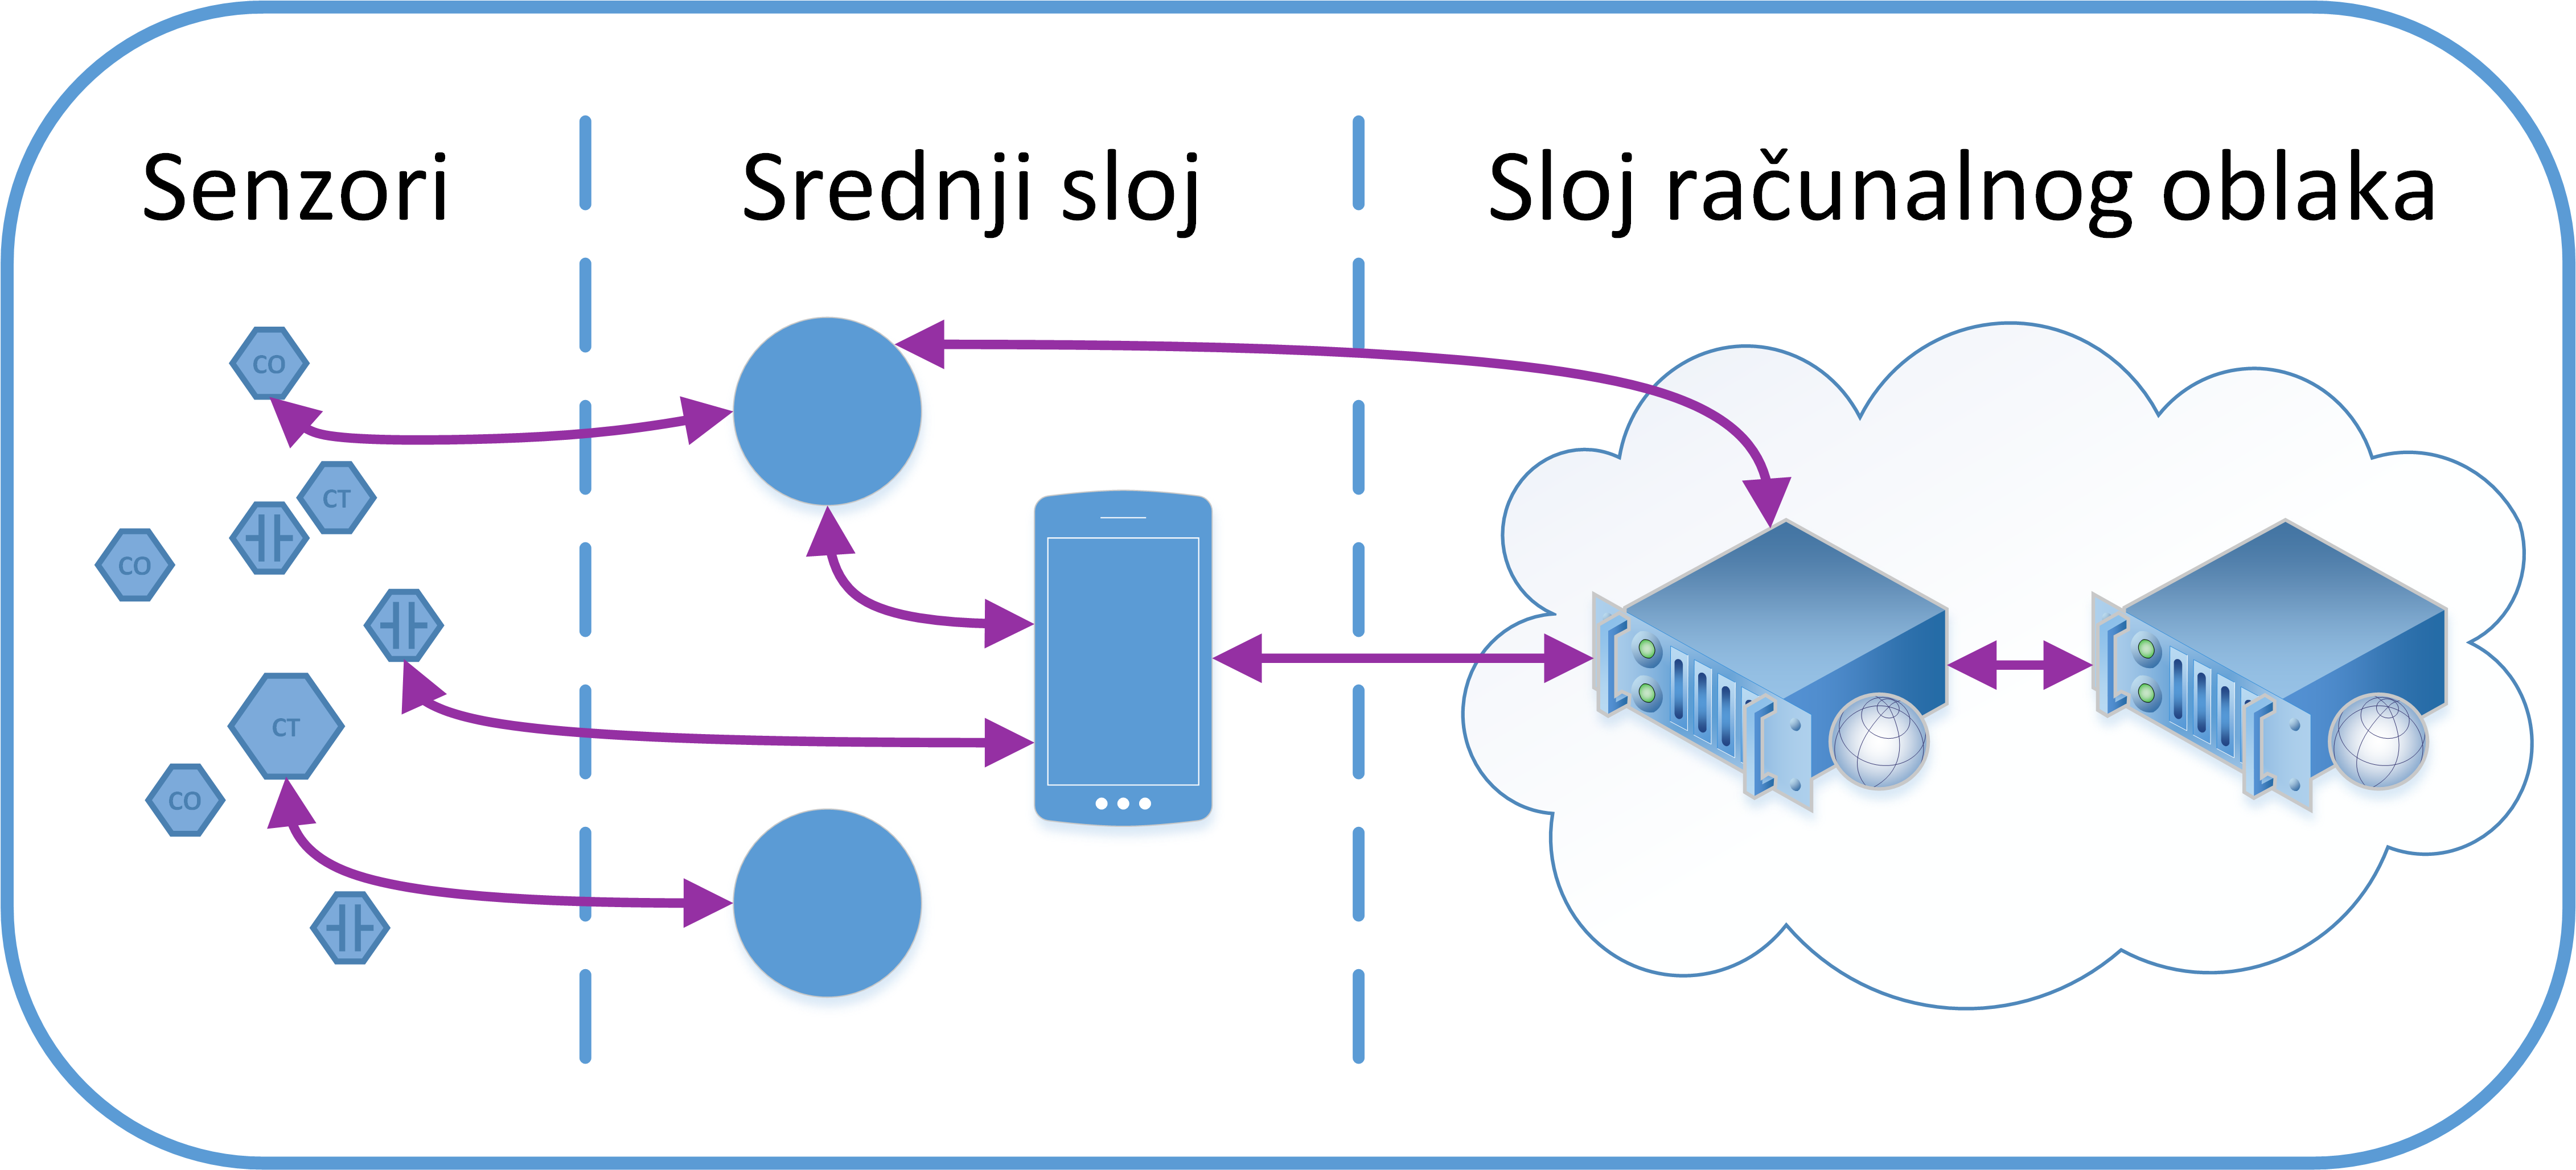
\includegraphics[width=\textwidth]{iot_independent}
        \caption{Arhitektura neovisna o platformi}
	\label{fig:independent}
    \end{subfigure}
    \begin{subfigure}[b]{0.49\textwidth}
        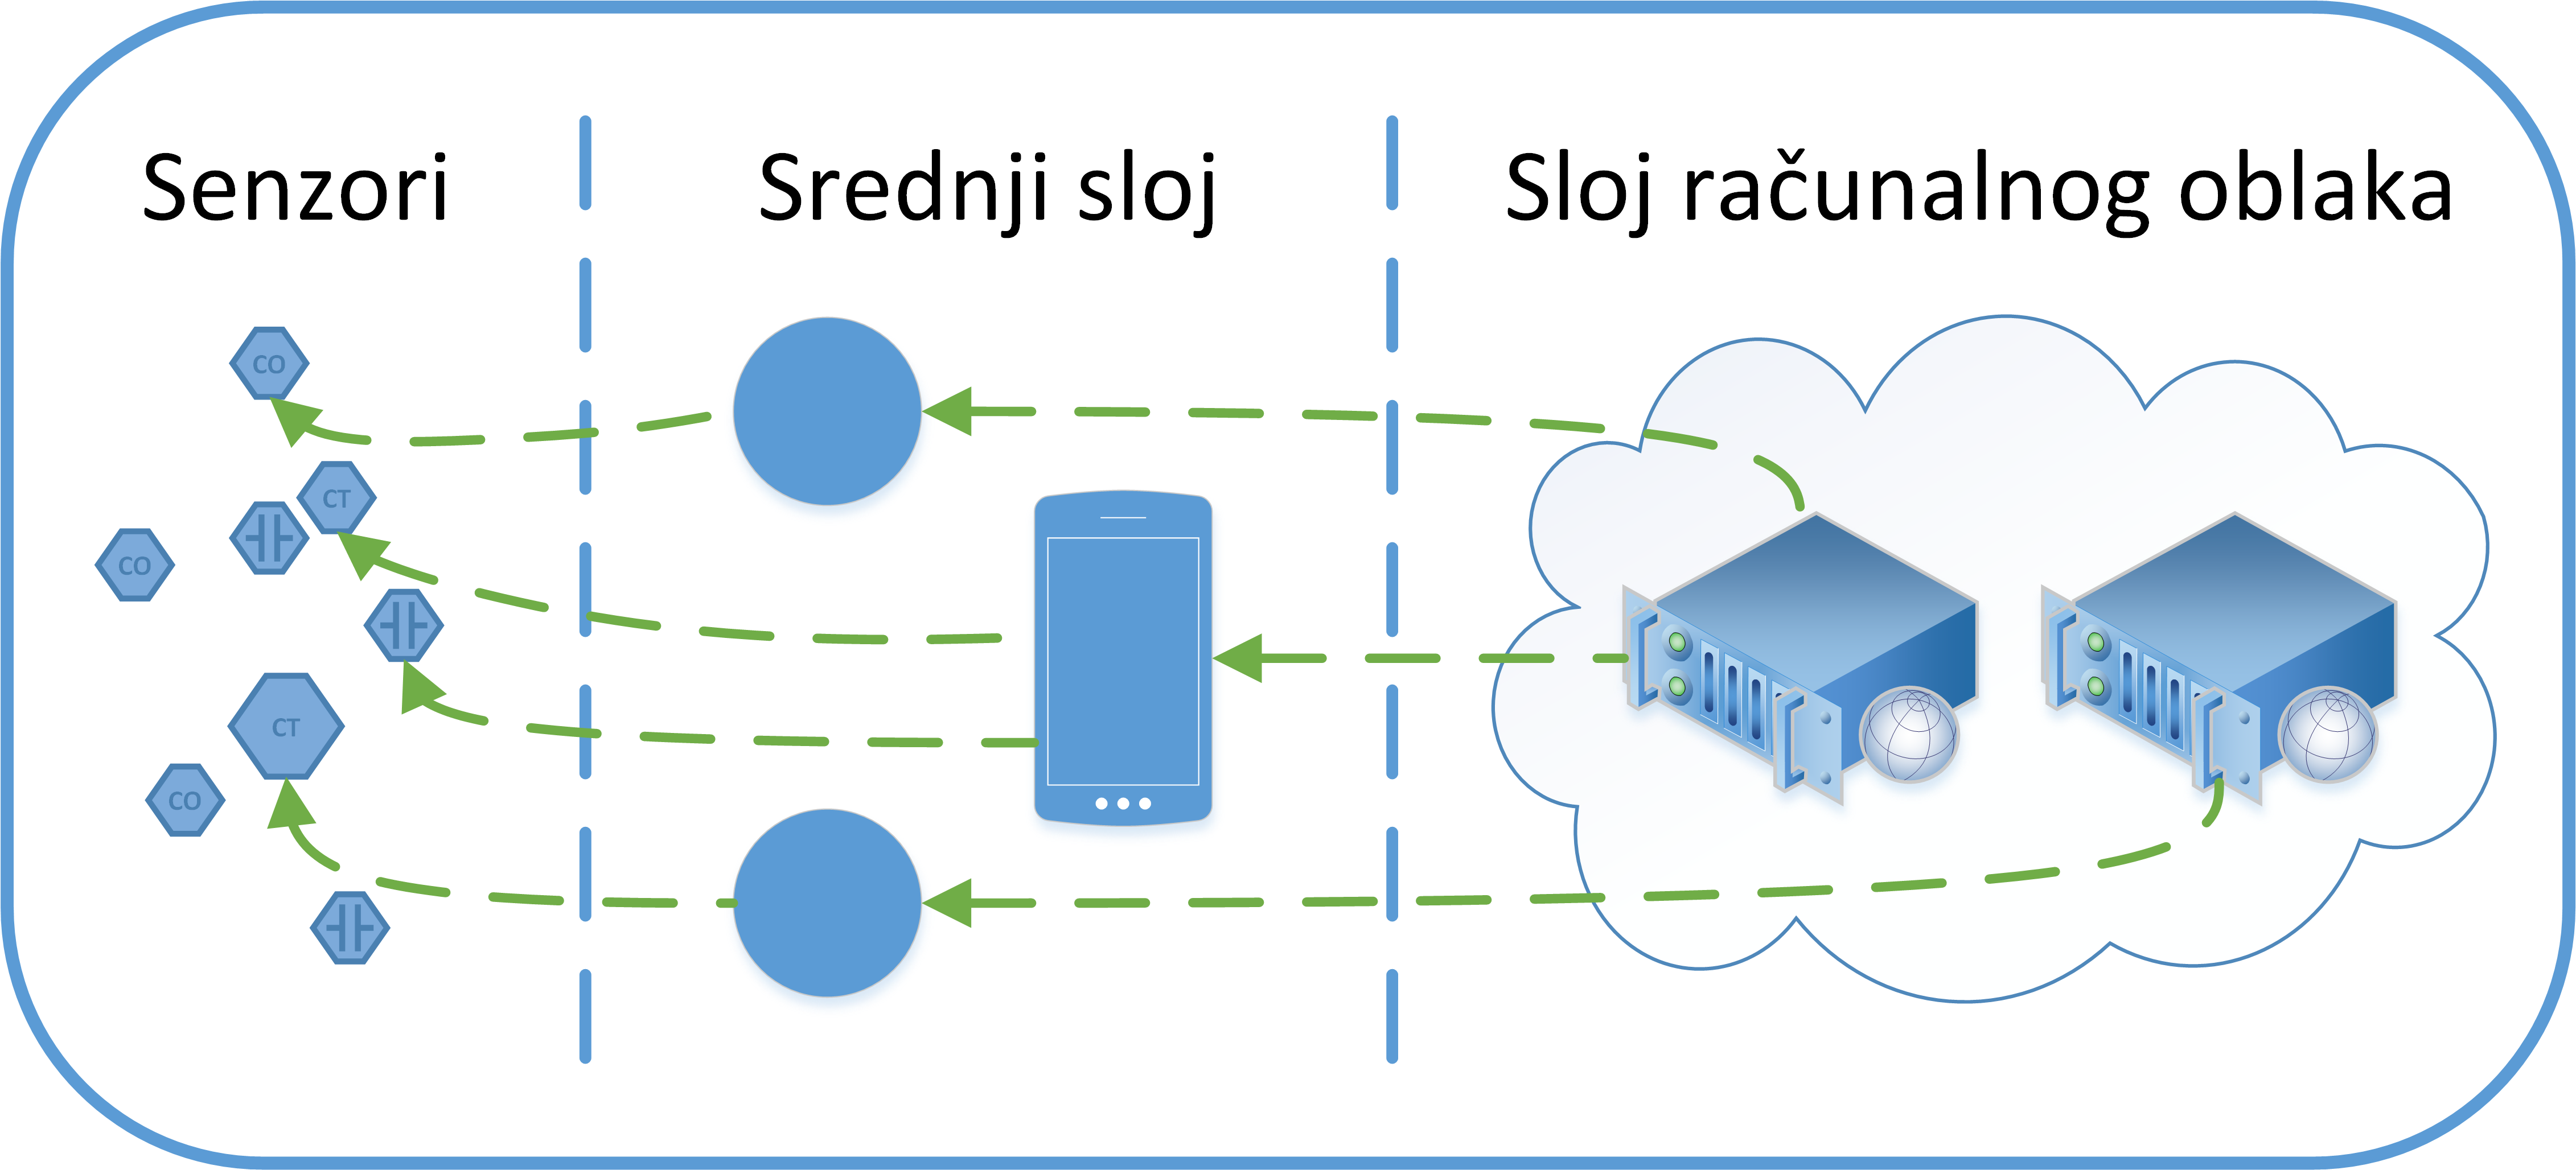
\includegraphics[width=\textwidth]{iot_authenticated}
        \caption{Autentificirano upravljanje uređajima}
	\label{fig:management}
    \end{subfigure}
    \begin{subfigure}[b]{0.49\textwidth}
        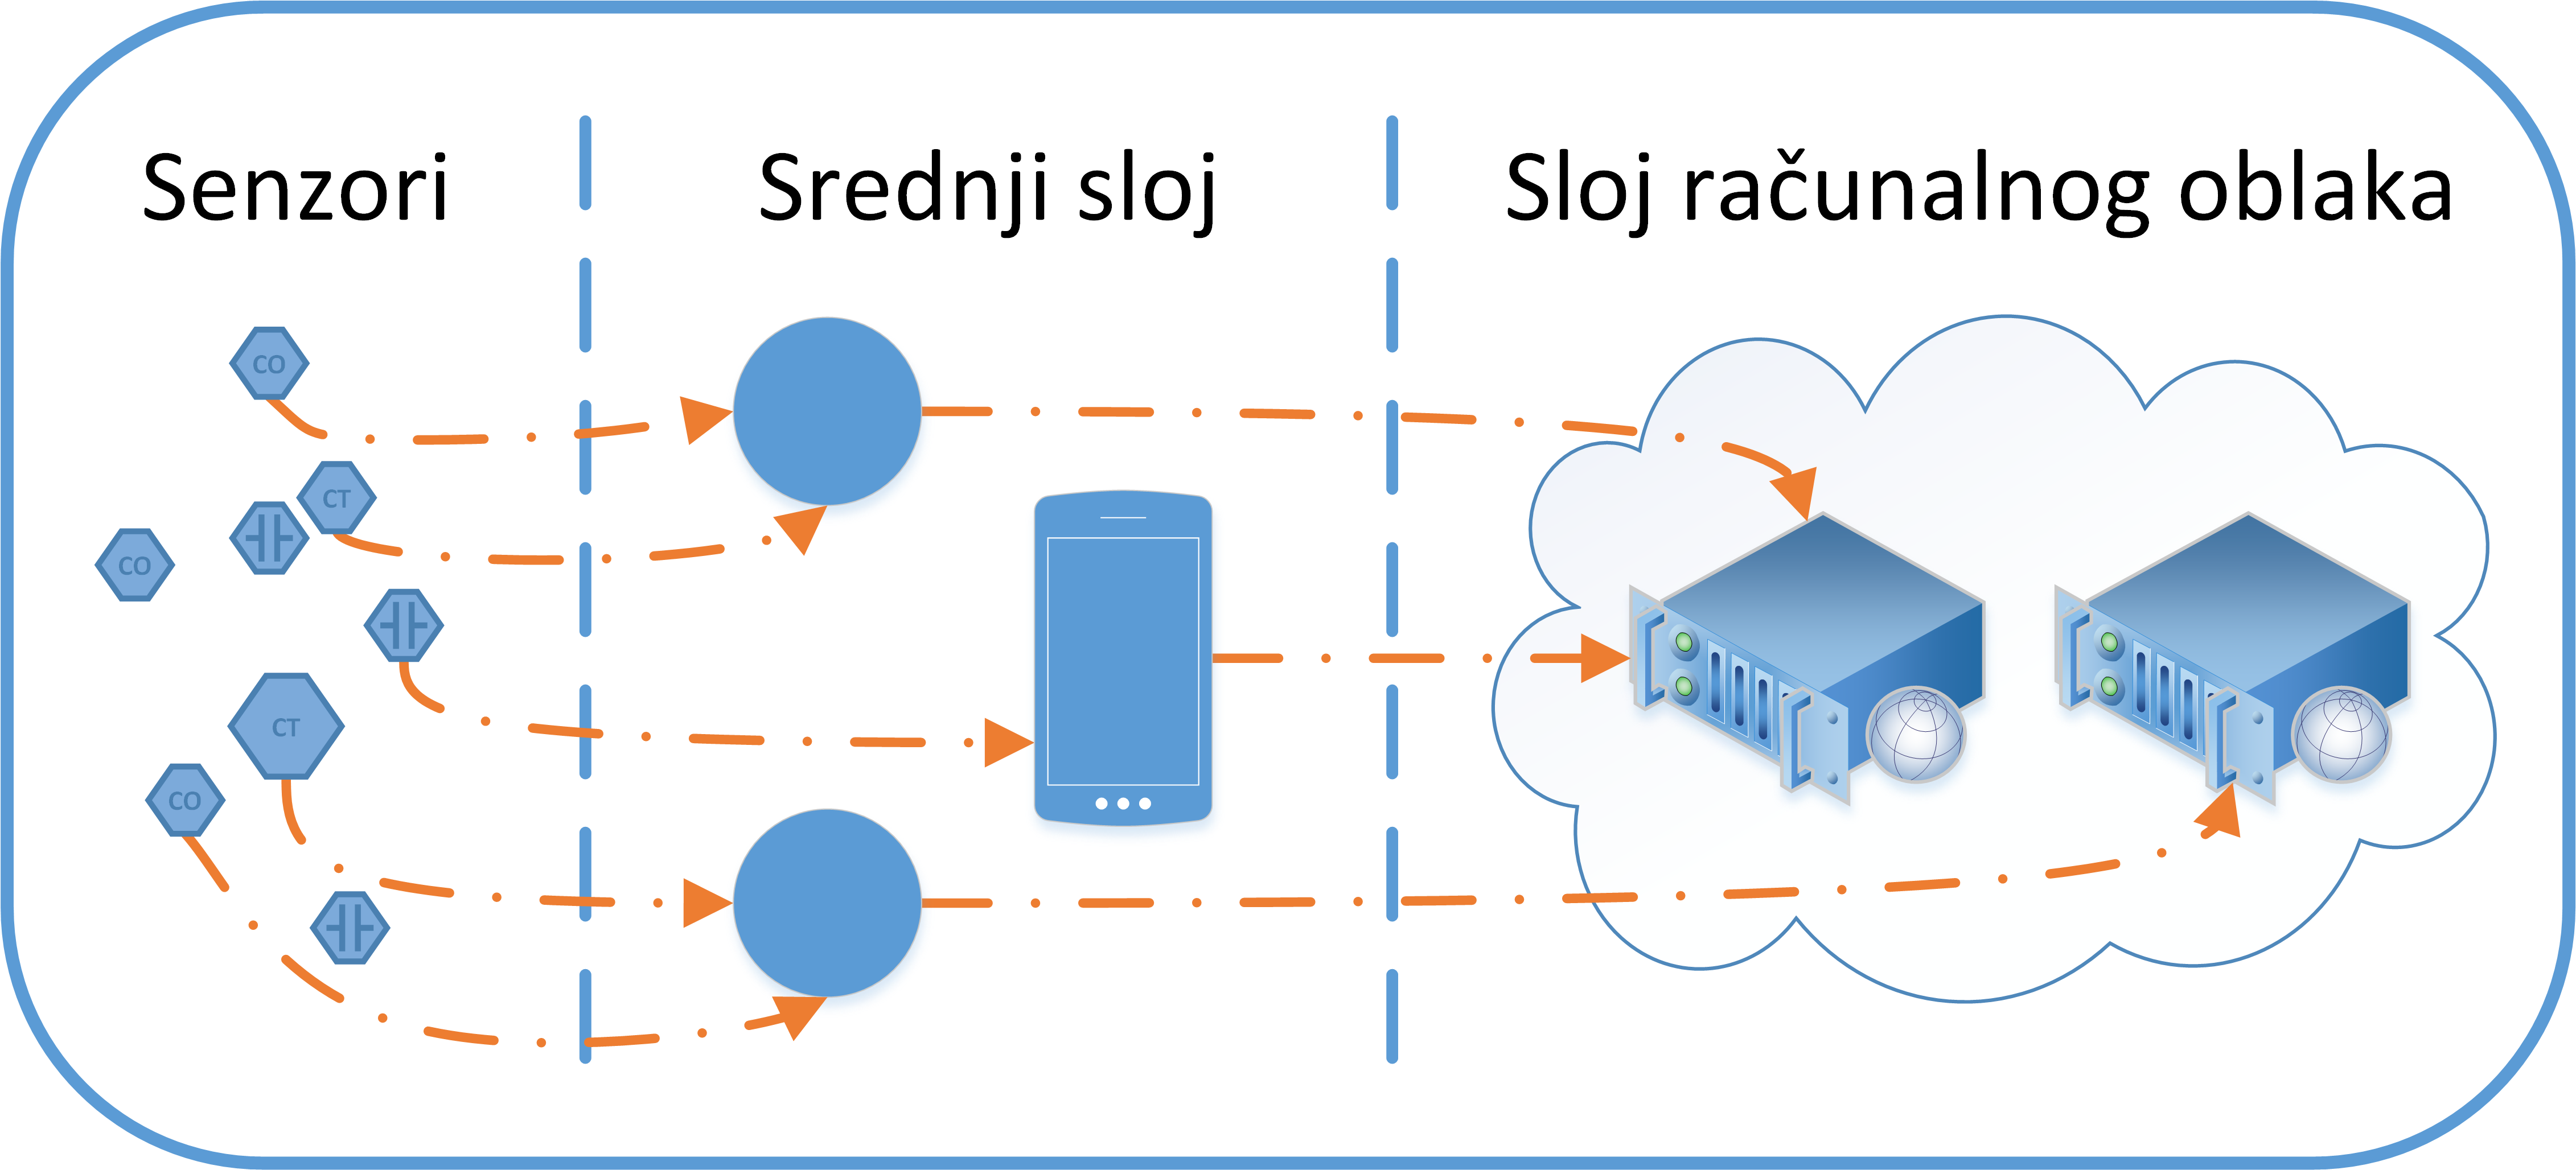
\includegraphics[width=\textwidth]{iot_reliable}
        \caption{Pouzdano prikupljanje podataka}
	\label{fig:reliable}
    \end{subfigure}
    \begin{subfigure}[b]{0.49\textwidth}
        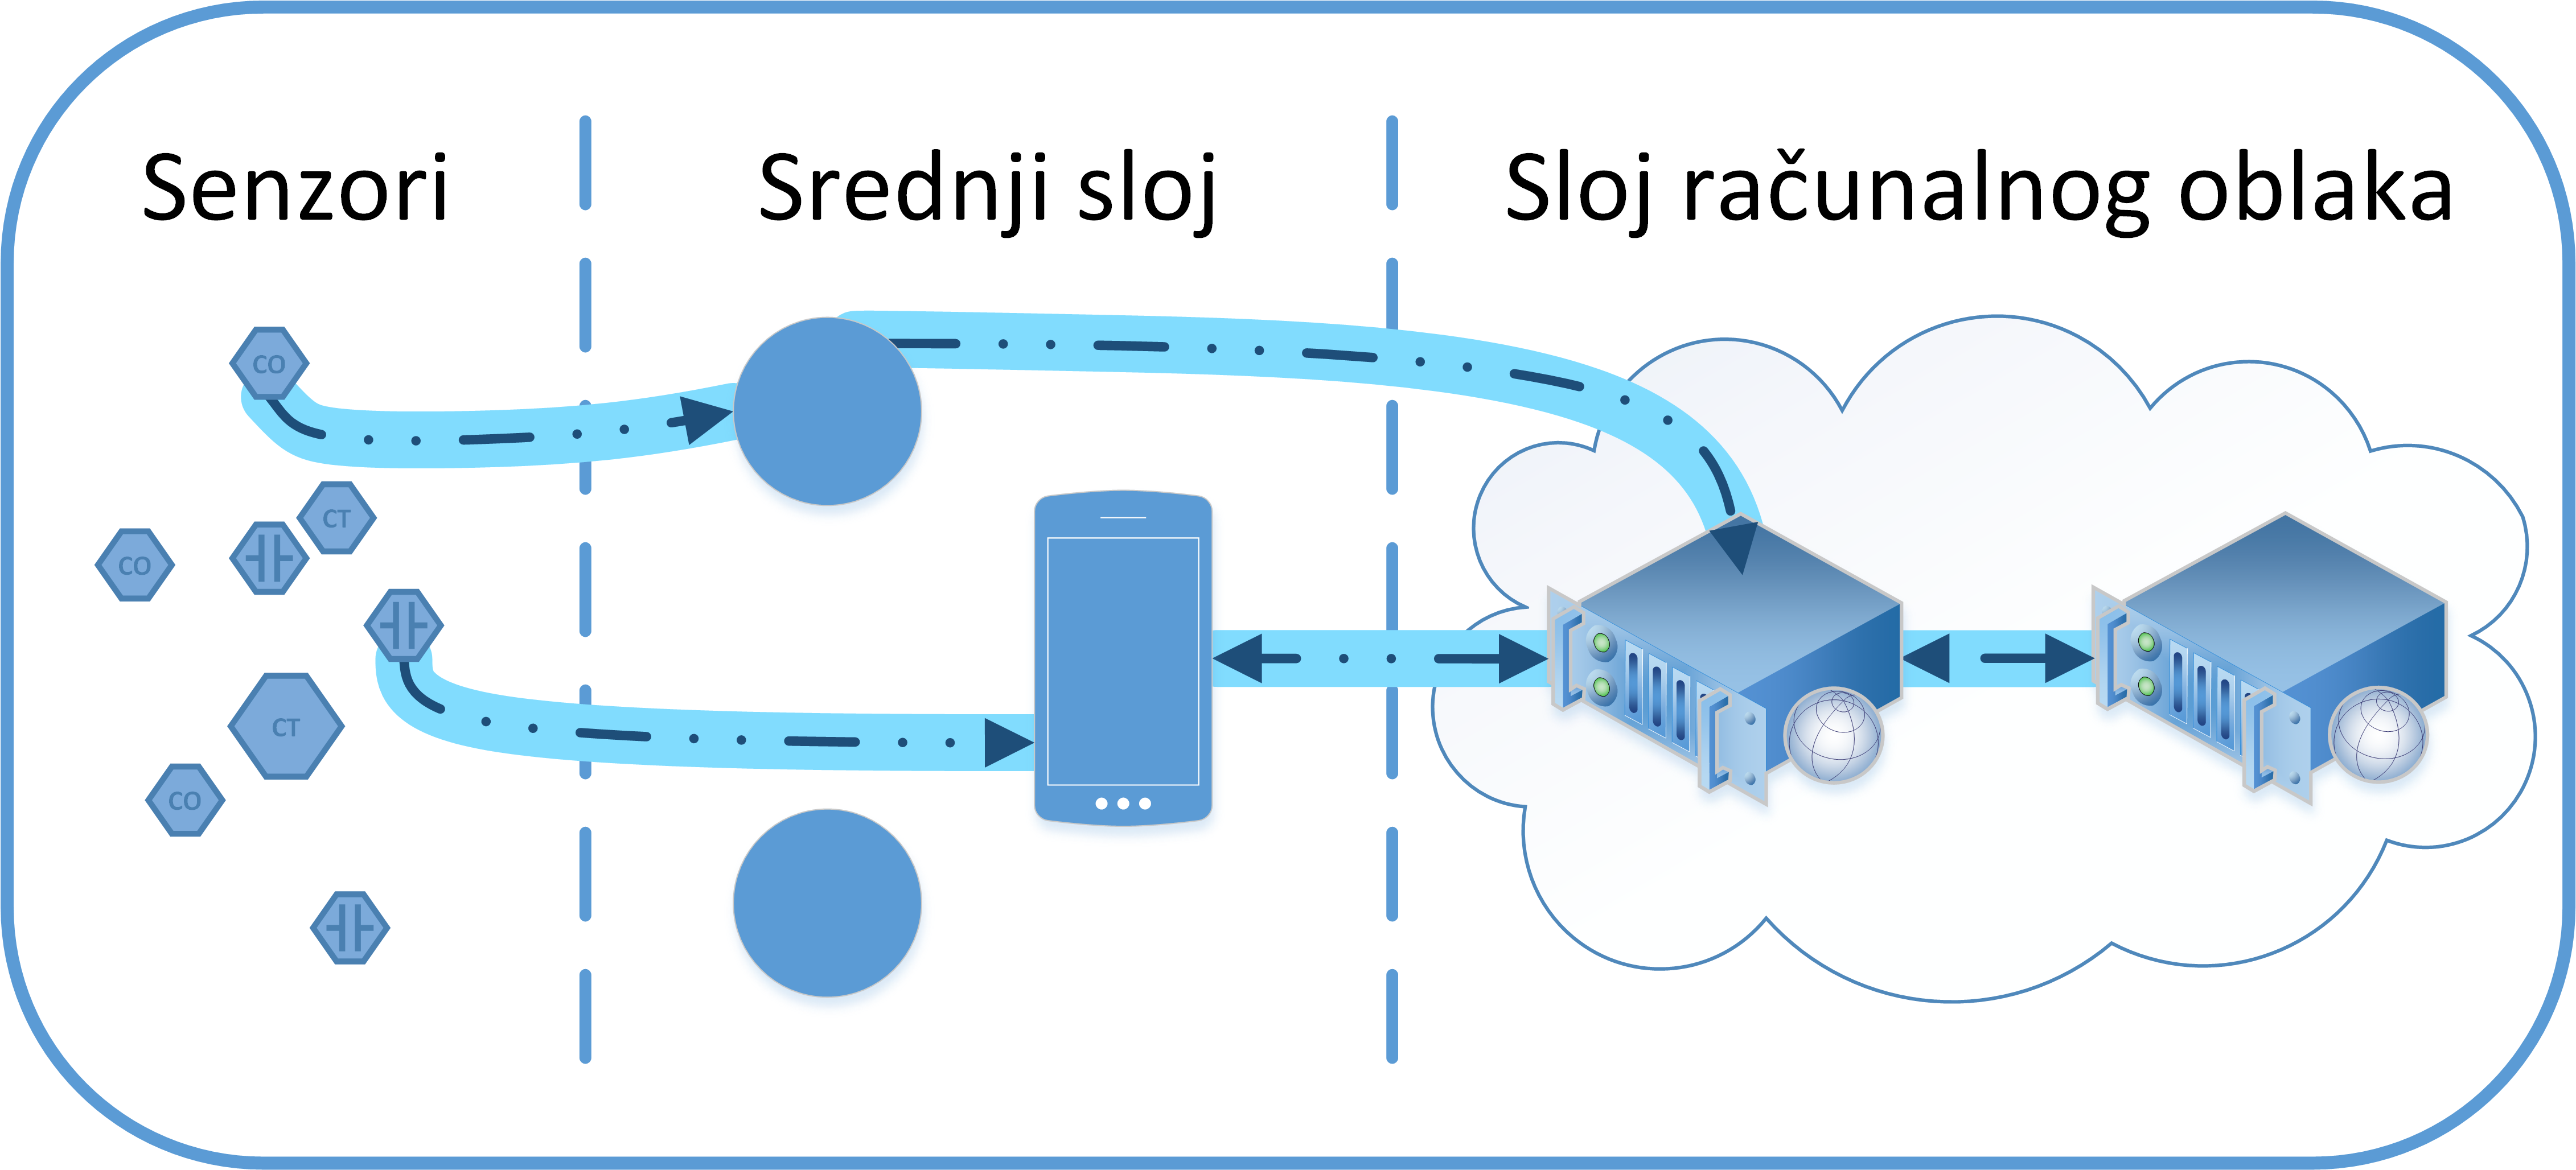
\includegraphics[width=\textwidth]{iot_sensitive}
        \caption{Zaštita osjetljivih podataka}
	\label{fig:sensitive}
    \end{subfigure}
    \caption{Primjene sigurne komunikacije u okolini Interneta stvari}
    \label{fig:iot}
\end{figure}

\subsection{Arhitektura neovisna o platformi} 
Neovisnost o platformi i uređajima u okolini Interneta stvari omogućena
je kroz uporabu prilagodljivog protokola ACAP za dogovor ključeva i algoritama koji
će se koristiti za zaštitu komunikacije. Protokol ACAP omogućuje dogovor u
oportunističkom mrežnom okruženju koje je karakteristično za Internet stvari i
podržava mogućnost dinamičke promjene kriptografskih algoritama i duljine
ključeva kako bi se ostvarila sigurnija komunikacija u slučaju ranjivosti ili
smanjilo opterećenje sustava u slučaju nedostatka resursa. Poruke u sustavu
mogu se razmjenjivati između dva uređaja ili biti proslijeđene od senzorskog
sloja sve do sloja računalnog oblaka, kako je prikazano na slici
\ref{fig:independent}. 

\subsection{Autentificirano upravljanje uređajima}
Svi uređaji, neovisno o sloju na kojem se nalaze, moraju imati sposobnost
autentifikacije kako bi se omogućilo pravilno upravljanje cijelog sustava
temeljenog na Internetu stvari. Upravljačke poruke obično dolaze iz sloja
računalnog oblaka i služe za prilagodbu uređaja u nižim slojevima arhitekture.
Tijek upravljačkih poruka prikazan je na slici \ref{fig:management}.
Autentifikacija upravljačkih poruka omogućava se tako da pošiljatelj
digitalno potpisuje poruke kako bi primatelj mogao provjeriti izvor poruke i
njenu cjelovitost. Digitalni potpis je računalno zahtjevna operacija i koristi
se samo za upravljačke poruke kako bi se uštedjelo na računalnim resursima.
Upravljačke poruke se, između ostalog, mogu koristiti za mijenjanje frekvencije
očitanja određenih senzora ili za slanje ažuriranja prema uređajima nižih
slojeva.

\subsection{Pouzdano prikupljanje podataka}
Uobičajeno je da se podaci prosljeđuju od izvora u nižim slojevima prema višim
slojevima. Tijekom prijenosa tih podataka napadač ima mogućnost presretanja
podataka i prosljeđivanja krivih mjerenja prema uređajima viših slojeva. To se
sprječava korištenjem HMAC zaštitne sume nad podacima koji se prosljeđuju. Time
je osigurana cjelovitost razmijenjenih poruka i omogućena pouzdanost
arhitekture. Pouzdani tok podataka za ovaj scenarij prikazan je na slici
\ref{fig:reliable}. Korištenje HMAC zaštitne sume umjesto digitalnog potpisa
omogućava značajno smanjenje složenosti operacija bez smanjivanja potrebne
razine sigurnosti (oba postupka omogućuju ostvarivanje sigurnosnog zahtjeva
cjelovitosti podataka). S obzirom na to da uređaji u sklopu senzorskog sloja imaju
pristup ograničenom izvoru napajanja, cilj je uštedjeti na potrošnji energije
prilikom zaštite podataka.
HMAC zaštita koristi se za prikupljanje podataka koji nisu osjetljivi (npr.
mjerenja kvalitete zraka ili vode), ali bi trebali biti vjerodostojni kako bi se
pružala kvalitetna usluga.

\subsection{Zaštita osjetljivih podataka}
U određenim scenarijima prikupljeni podaci mogu biti osjetljive prirode i
trebaju se zaštiti tako da sprječavaju curenje podataka kao što je prikazano
na slici \ref{fig:sensitive}. Potreba za zaštitom podataka može se pojaviti u
komunikaciji između svih slojeva u sklopu arhitekture. Iako senzori najčešće
prikupljaju neosjetljive podatke, određene primjene, poput sustava za
praćenje tjelesnog zdravlja, ne bi smjele dozvoljavati uvid u izmjerene podatke.
Isto tako, određene korporativne primjene zahtijevaju da svi podaci unutar
arhitekture budu tajni kako se ne bi otkrivali osjetljivi podaci o korisnicima
sustava. Zaštita osjetljivih podataka postiže se simetričnom kriptografijom,
odnosno šifriranjem podataka na izvoru i dešifriranjem na odredištu korištenjem
prethodno razmijenjenog tajnog ključa.

\section{Model sigurne komunikacije u okolini Interneta stvari}

Model sigurne komunikacije u okolini Interneta stvari definiran je kao šestorka
$S_{IoT}$:

\begin{equation}
    S_{IoT}=\{D,K,L,C,A,O\},
\end{equation}

gdje je $D$ skup svih uređaja (engl. \emph{devices}), $K$ skup svih parova
ključeva (privatnog i odgovarajućeg javnog ključa)
svih uređaja, $L$ je skup svih komunikacijskih slojeva (engl.
\emph{communication layers}) na kojem uređaji mogu komunicirati, $C$ skup svih
mogućnosti uređaja (engl. \emph{capabilities}), $A$ je skup kriptografskih
algoritama koje uređaji mogu koristiti i $O$ je skup operacija
s kojima se ostvaruje sigurna komunikacija između uređaja.

Za potrebe ovog modela razlikujemo tri različite vrste kriptografskih
algoritama u sklopu skupa $A=\{A^h,A^s,A^p\}$: algoritme kriptografskog sažetka
$A^h$, simetrične algoritme $A^s$ i asimetrične algoritme $A^p$.

Uređaj $D_i$ u modelu je označen sa svojim skupom podržanih
komunikacijskih slojeva $L_i$, skupom hardverskih mogućnosti $C_i$, skupom
podržanih kriptografskih algoritama $A_i$ i skupom parova javnih i privatnih
ključeva $K_i$:
\begin{equation}
    D_i \in D:\{D_i=\{L_i,C_i,A_i,K_i\},\ L_i \subseteq L,\ C_i \subset C,\ A_i 
    \subseteq A,\ K_i \subset K\},
\end{equation}
gdje je $A_i=\{A^h_i,A^s_i,A^p_i\}$ takav da vrijedi $A^h_i\subseteq A^h$,
$A^s_i\subseteq A^s$ i $A^p_i\subseteq A^p$.

Svaki par ključeva $k(a^p_i)\in K_i$ stvara se tako da odgovara asimetričnom
algoritmu $a^p_i\in A^p_i$. Par ključeva $k(a^p_i)$ 
sadrži privatni ključ $pri(a^p_i)$
i njemu odgovarajući javni ključ $pub(a^p_i)$:
\begin{equation}
    k(a^p_i)=\{pri(a^p_i), pub(a^p_i)\}.
\end{equation}

Skup javnih ključeva za svaki uređaj mora se prebaciti na drugi uređaj prilikom
uspostave sigurne komunikacije.
Skup javnih ključeva $PK_i$ za uređaj $D_i$ definiran je kao: 
\begin{equation}
PK_i=\{pub(a^p_i)\in k(a^p_i):k(a^p_i)\in K_i\}.
\end{equation}

U predloženom modelu, dva uređaja $D_i$ i $D_j$ mogu komunicirati samo
ako imaju zajednički komunikacijski sloj na kojem mogu komunicirati, odnosno ako
vrijedi sljedeće: $L_i \cap L_j \neq \emptyset$.
Komunikacijski sloj definira vrstu sučelja i mrežne protokole koji se mogu
koristiti za razmjenu podataka između uređaja (npr. WLAN, Ethernet, IP, TCP,
UDP). 

\no{
Note that a typical device from the perceptual 
tier has a wireless interface (e.g. Bluetooth or Zigbee) for interaction with a 
intermediate tier device, while the latter device uses a high speed communication 
interface (e.g. WLAN or Ethernet) to communicate with the cloud tier.
}

Za ostvarivanje sigurne komunikacije između uređaja u predloženom modelu
definira se skup operacija $O$ koji se sastoji od šest operacija namijenjenih
sigurnoj komunikaciji koje se koriste za dogovor algoritama i ključeva,
osiguravanje cjelovitosti podataka, autentifikaciju i tajnost podataka.
\begin{equation}
    O=\{dogovor, \mathit{potpis}, \mathit{provjera\_potpisa}, hmac, \mathit{sifriranje}, \mathit{desifriranje}\}
\end{equation}

Operacija dogovora kriptografskih algoritama i zajedničke tajne
(\textit{dogovor}) je preduvjet za daljnju sigurnu komunikaciju između
klijenta (započinjatelja) $D_i$ i poslužitelja (odgovaratelja) $D_j$ i mora biti
provedena prije svih drugih
operacija. Ova operacija dogovora predstavlja protokol ACAP koji služi za
dogovor oko preduvjeta sigurne komunikacije. Rezultat operacije je trojka
kriptografskih algoritama ($\widetilde{A}_{ij}$) koja se može koristiti na oba
uređaja, zajednička tajna ($S_{ij}$) koju se može koristiti za stvaranje novih
tajnih ključeva za zaštitu podataka i javni ključ svakog uređaja:
\begin{equation}
	dogovor:(D_i,D_j)\longmapsto\{\widetilde{A}_{ij},S_{ij},pub(a^p_i),pub(a^p_j)\},
	\label{eq:agreement}
\end{equation}
gdje vrijedi da je
$\widetilde{A}_{ij}=\{\widetilde{A}^h_{ij},\widetilde{A}^s_{ij},\widetilde{A}^p_{ij}\}$
takav da je $\widetilde{A}^h_{ij}\in A^h_{i}\cap A^h_{j}$,
$\widetilde{A}^s_{ij}\in A^s_{i}\cap A^s_{j}$ i $\widetilde{A}^p_{ij}\in
A^p_{i}\cap A^p_{j}$. 

Drugim riječima, dogovoreni algoritmi kriptografskog sažetka, simetrične i
asimetrične kriptografije moraju biti podržani na oba uređaja.
Javni ključevi $pub(a^p_i)$ i $pub(a^p_j)$ odgovaraju dogovorenom algoritmu
asimetrične kriptografije $\widetilde{A}^p_{ij}$ tako da vrijedi
$a^p_i=a^p_j=\widetilde{A}^p_{ij}$. Do zajedničke tajne $S_{ij}$ dolazi se s
pomoću Diffie-Hellman izračuna opisanog u poglavlju \ref{sec:dh}.


U modelu definirane su sljedeće sigurne komunikacijske operacije koje se
mogu izvoditi samo nakon uspješne operacije dogovora:
\begin{itemize}  
    \item Zaštita cjelovitosti podataka uz neporecivost (\textit{potpis}) u obliku
	digitalnog potpisa za podatke koje se razmjenjuju između pošiljatelja
	$D_i$ i primatelja $D_j$:
	\begin{equation}
	    \mathit{potpis}:[podaci,\widetilde{A}^h_{ij},\widetilde{A}^p_{ij},pri(a^p_i)]\longmapsto\{\mathit{digitalni\_potpis}\}.
	    \label{eq:sign}
	\end{equation}
	    
	Digitalni potpis računa se iz podataka kroz izračun
	kriptografskog sažetka dogovorenim algoritmom $\widetilde{A}^h_{ij}$ te
	asimetričnom operacijom potpisivanja korištenjem algoritma
	$a^p_i=\widetilde{A}^p_{ij}$ i odgovarajućeg privatnog ključa
	$pri(a^p_i)$. Uređaj $D_j$ po primitku podataka provjerava valjanost
	digitalnog potpisa korištenjem operacije $provjera\_potpisa$:
	\begin{equation}
	    \mathit{provjera\_potpisa}:[\{podaci,\mathit{potpis}\},\widetilde{A}^h_{ij},\widetilde{A}^p_{ij},pub(a^p_i)]\longmapsto~[ispravan,neispravan]
	\end{equation}
	Primatelj $D_j$ provjerava dobiveni digitalni potpis tako
	da uspoređuje rezultat kriptografskog sažetka s algoritmom
	$\widetilde{A}^h_{ij}$ nad dobivenim podacima,
	s dešifriranim kriptografskim sažetkom iz digitalnog potpisa
	algoritmom $a^p_j=\widetilde{A}^p_{ij}$ i odgovarajućim
	javnim ključem $pub(a^p_i)$. Ako se sažeci podudaraju potpis je
	ispravan, u suprotnom potpis je neispravan.

    \item Autentifikacija podataka i zaštita cjelovitosti algoritmom HMAC
	(\textit{hmac}) koristi se kao jednostavniji mehanizam zaštite koji
	zahtijeva manje resursa od digitalnog potpisa. Operacija \emph{hmac}
	prilikom slanja podataka $data$ između pošiljatelja $D_i$ i primatelja
	$D_j$ definirana je na sljedeći način:
	\begin{equation}
	    hmac:(podaci,\widetilde{A}^h_{ij},S_{ij})\longmapsto\{za\breve{s}titna\_suma\}
	    \label{eq:hmac}
	\end{equation}
	
	Zaštitna suma se računa korištenjem dogovorenog algoritma kriptografskog
	sažetka $\widetilde{A}^h_{ij}$ s dogovorenom zajedničkom tajnom $S_{ij}$
	nad podacima koji se šalju.
	Primatelj $D_j$ uspoređuje dobivenu zaštitnu sumu sa zaštitnom sumom
	izračunatom nad dobivenim podacima s istim ključem. Provjera zaštitne
	sume je uspješna ako se primljena i izračunata zaštitna suma podudaraju.
	
    \item Tajnost podataka korištenjem operacija \textit{sifriranje} i
	\textit{desifriranje} za podatke razmijenjene između pošiljatelja $D_i$
	i primatelja $D_j$. Operacija šifriranja koristi prethodno dogovoreni
	algoritam simetrične kriptografije $\widetilde{A}^s_{ij}$ i zajedničku
	tajnu $S_{ij}$ nad podacima:
	\begin{equation}
	    \mathit{sifriranje}:(podaci,\widetilde{A}^s_{ij},S_{ij})\longmapsto~\mathit{tajni\_podaci}
	\end{equation}
	Izvorni podaci se izračunavaju s operacijom dešifriranja uz korištenje
	istog algoritma i zajedničke tajne:
	\begin{equation}
	    \mathit{desifriranje}:(\mathit{tajni\_podaci},\widetilde{A}^s_{ij},S_{ij})\longmapsto~podaci
	\end{equation}
\end{itemize}

Predstavljeni model sigurne komunikacije je minimalan skup objekata i operacija
koje su potrebne za sigurnu komunikaciju između svih uređaja unutar okoline
Interneta stvari neovisno o njihovim mogućnostima.

\section{Prilagodljivost modela sigurne komunikacije}
\label{sec:iotprilag}

Predloženi model je prilagodljiv jer podržava različite načine dogovora
korištenih algoritama ovisno o trenutnim mogućnostima uređaja $D_i$ i $D_j$. Za
odabir algoritama koristi se poopćenje procedure koja je definirana u poglavlju
\ref{sec:dogovor}, a temeljeno je na protokolu SSH \ref{sec:ssh}. Protokol SSH
uzima u
obzir samo redoslijed algoritama u popisu, odnosno pretpostavlja da će
algoritmi biti poredani po sigurnosti ili brzini izvođenja. Osnovni
nedostatak tog pristupa je nemogućnost dinamičke promjene uvjeta odabira.

\no{Predložena procedura je poopćena inačica postupka koji se koristi u sklopu protokola SSH prikazanog u poglavlju \ref{sec:ssh}. Protokol SSH pretpostavlja najvišu razinu sigurnosti i ne uzima u obzir računalne sposobnosti komunicirajućih strana. Ukoliko je kriptografski algoritam implementiran, on će se koristiti neovisno o mogućem utjecaju na brzinu obrade zaštićenih podataka.}

Za područje Interneta stvari prikladan je unaprijeđeni algoritam dogovora koji je
prikazan u algoritmu \ref{alg:agreement2}, a omogućuje dinamičko
odlučivanje oko algoritma koji će se koristiti ovisno o trenutnim sposobnostima
komunicirajućih strana.
Osnova za vrednovanje algoritama leži u odlučivanju koji je algoritam
primjereniji za upotrebu ovisno o uvjetima u kojima se odvija sigurna
komunikacija. Vrijednost algoritma može biti povezana izravno s mjerljivim
mogućnostima komunicirajućih uređaja, poput računalne moći, propusnosti
komunikacije ili pristupa izvoru napajanja.

\begin{algorithm}
\caption{Procedura za dogovor kriptografskih algoritama}
\label{alg:agreement2}
\begin{algorithmic}[1]
    \Procedure{Crypto\textendash Agreement}{$C_i$, $C_j$, $A_i$, $A_j$, $rsig$}\
    \For{svaka $vrsta \in \{h,s,p\}$}
    \For{svaki $a^{vrsta} \in (A^{vrsta}_i \cap A^{vrsta}_j)$}
    \If{($\widetilde{A}^{vrsta}_{ij} == \varnothing$) \textbf{or} 
    $(score(a^{vrsta},C_i,C_j,rsig) > score(\widetilde{A}^{vrsta}_{ij},C_i,C_j, rsig))$}
		\State $\widetilde{A}^{vrsta}_{ij}$ = $a^{vrsta}$
		\State \textbf{break}
	    \EndIf
	\EndFor
	\If{$\widetilde{A}^{vrsta}_{ij} == \varnothing$}
	\State \Return $\varnothing$ \Comment Dogovor je neuspješan jer nema zajedničkih algoritama.
	\EndIf
    \EndFor
    \State \Return 
    $\widetilde{A}_{ij}=\{\widetilde{A}^{h}_{ij},\widetilde{A}^{s}_{ij},\widetilde{A}^{a}_{ij}\}$
\EndProcedure
\end{algorithmic}
\end{algorithm}

Algoritam uzima u obzir mogućnosti klijenta i poslužitelja $C_i$ i $C_j$ te
potrebnu razinu sigurnosti $rsig$ kako bi iz popisa podržanih algoritama
$A_i$ i $A_j$ odabrao prikladne algoritme ovisno o trenutnim mogućnostima (linija 1).

Procedura dogovora prolazi kroz sve vrste algoritama koje su potrebne za
osiguravanje daljnje komunikacije (hash - $h$ , simetrični - $s$, asimetrični - $p$)
(linija 2-12) i za svaku vrstu odabire algoritam $a^{vrsta}$ iz presjeka
algoritama obje strane ($A^{vrsta}_i \cap A^{vrsta}_j$). Odabire se algoritam
koji ima najveću
vrijednost u odnosu na ostale algoritme (linije 3-8). Vrijednost pojedinog
algoritma određuje
se s pomoću funkcije za računanje vrijednosti $score(a^{vrsta},C_i,C_j,rsig)$
(linija 4). Konačno, procedura vraća n-torku odabranih algoritama (linija 13)
ili prazan skup (linija 10) koji predstavlja neuspješan dogovor. Predložena
procedura za dogovor je ostvarena uz pretpostavku da je razina sigurnosti
najvažniji parametar. U tom slučaju se ova procedura može poistovjetiti s
procedurom za odabir u protokolu SSH.

Prilikom postavljanja cjelokupne okoline za sigurnu komunikaciju potrebno je
izmjeriti podatke o mogućnostima uređaja koji sudjeluju u komunikaciji i prema
tome odrediti parametre za funkciju vrednovanja $score$.
Funkcija $score$ za vrednovanje algoritama omogućuje fleksibilno definiranje
vrijednosti ovisno o pojedinoj primjeni. U okolini Interneta stvari važno je
uzeti u obzir trenutne mogućnosti uređaja i prema tome odrediti koji je
algoritam najbolji, a koji najgori u danom trenutku. Ukupna vrijednost algoritma
$a$, koja je definirana izrazom $score(a,C_i,C_j,rsig)$, zapravo je
kombinacija vrijednosti u više dimenzija. Osnovne dimenzije dolaze od trenutno
zahtjevane razine sigurnosti $rsig$, računalne zahtjevnosti algoritma $ac$
(engl. \emph{algorithm complexity}) i trenutnih mogućnosti oba uređaja koje
obuhvaćaju trenutnu razinu napajanja $bp$ (engl. \emph{battery power}),
propusnosti komunikacijske veze $bw$ (engl. \emph{bandwidth}) i računalne snage
uređaja $pp$ (engl. \emph{processing power}):
\vspace{-10pt}
\begin{multline}
    score(a,C_i,C_j,rsig)=\\f[w_{0}\cdot rsig, w_{1}\cdot ac(a), 
	w_{2}\cdot min(bp_i,bp_j), 
    w_{3}\cdot min(bw_i,bw_j), w_{4}\cdot min(pp_i,pp_j)],
\end{multline}
gdje su $C_i$ i $C_j$ redom definirani kao $\{bp_i,bw_i,pp_i\}$ i
$\{bp_j,bw_j,pp_j\}$. Različite težine $w_x$ ukazuju na relativnu važnost
i definiraju doprinos određene dimenzije u odnosu na cjelokupnu vrijednost
algoritma. Odnosi težina se određuju na temelju trenutne primjene i okoline u
kojoj je sustav postavljen. Prioritet se daje uređaju koji trenutno ima manju
razinu mogućnosti (funkcija $\min$).

\subsection{Prilagodbe odabira algoritma}

Funkcija za vrednovanje $score$ omogućuje prilagodljivost procedure za dogovor
na razne uvjete komunikacije ovisno o namjeni i ograničenjima sustava.
Primjerice:
\begin{itemize}
    \item Ako se radi o sustavu koji prikuplja i obrađuje velike količine
	podataka, najveća težina će se postaviti na propusnost komunikacijske
	veze $bw_x$ i na računalnu zahtjevnost algoritma $ac_x$ kako se podaci
	mogli sigurno prikupljati zavodoljavajućom brzinom.
    \item U slučaju postavljanja sustava za dugoročno prikupljanje, težina će
	biti postavljena na trenutnu razinu napajanja $bw_x$.
    \item Kod postavljanja sustava s visokim zahtjevima na sigurnost, težina će
	se postaviti na razinu sigurnosti komunikacije $rsig$, a drugi ključni
	parametar će biti računalna snaga uređaja $pp_x$.
\end{itemize}

Prilikom specifikacije funkcije vrednovanja važno je odrediti što je prioritet
kod postavljanja sustava. U slučaju da imamo sustav za prikupljanje podataka o
temperaturi na određenom području, važno je odrediti kroz koji će se period
prikupljati očitanja i procijeniti trošak obrade pojedinog mjerenja koji
uključuje mjerenje, zaštitu podataka i slanje podataka. Različiti algoritmi
će imati različitu zahtjevnost, odnosno potrošnju električne energije. Stoga je
važno pravilno izmjeriti težinu pojedinog algoritma za uređaj koji se postavlja
i definirati računalne zahtjevnosti za svaki algoritam.

Ako se za vrijeme rada sustava promijene zahtjevi na sigurnost ili se postave
drukčiji prioriteti na težinu određenih parametara, moguće je s viših slojeva
ažurirati težine tih parametara i prilagoditi sustav trenutnim potrebama. Na taj
način bi se mogla smanjiti učestalost očitanja kako bi se uštedjela energija
potrebna za omogućavanje tajnosti očitanih podataka.

Prilikom komunikacije dva uređaja s različitih slojeva, prioritet kod izračunavanja
funkcije vrednovanja daje se uređaju koji se nalazi na nižem sloju arhitekture.
Na taj se način štede resursi u nižim slojevima arhitekture kako bi se
prikupljanje podataka obavilo na što efikasniji način.

% vim: spell spelllang=hr
